\documentclass[border=10pt]{standalone}
\usepackage[svgnames]{xcolor}
\usepackage{amsmath}
\usepackage{pgfplots}
\pgfplotsset{compat=newest}
\usepackage[sfdefault]{FiraSans}
\usepackage{FiraMono}
\renewcommand*\familydefault{\sfdefault}
\begin{document}
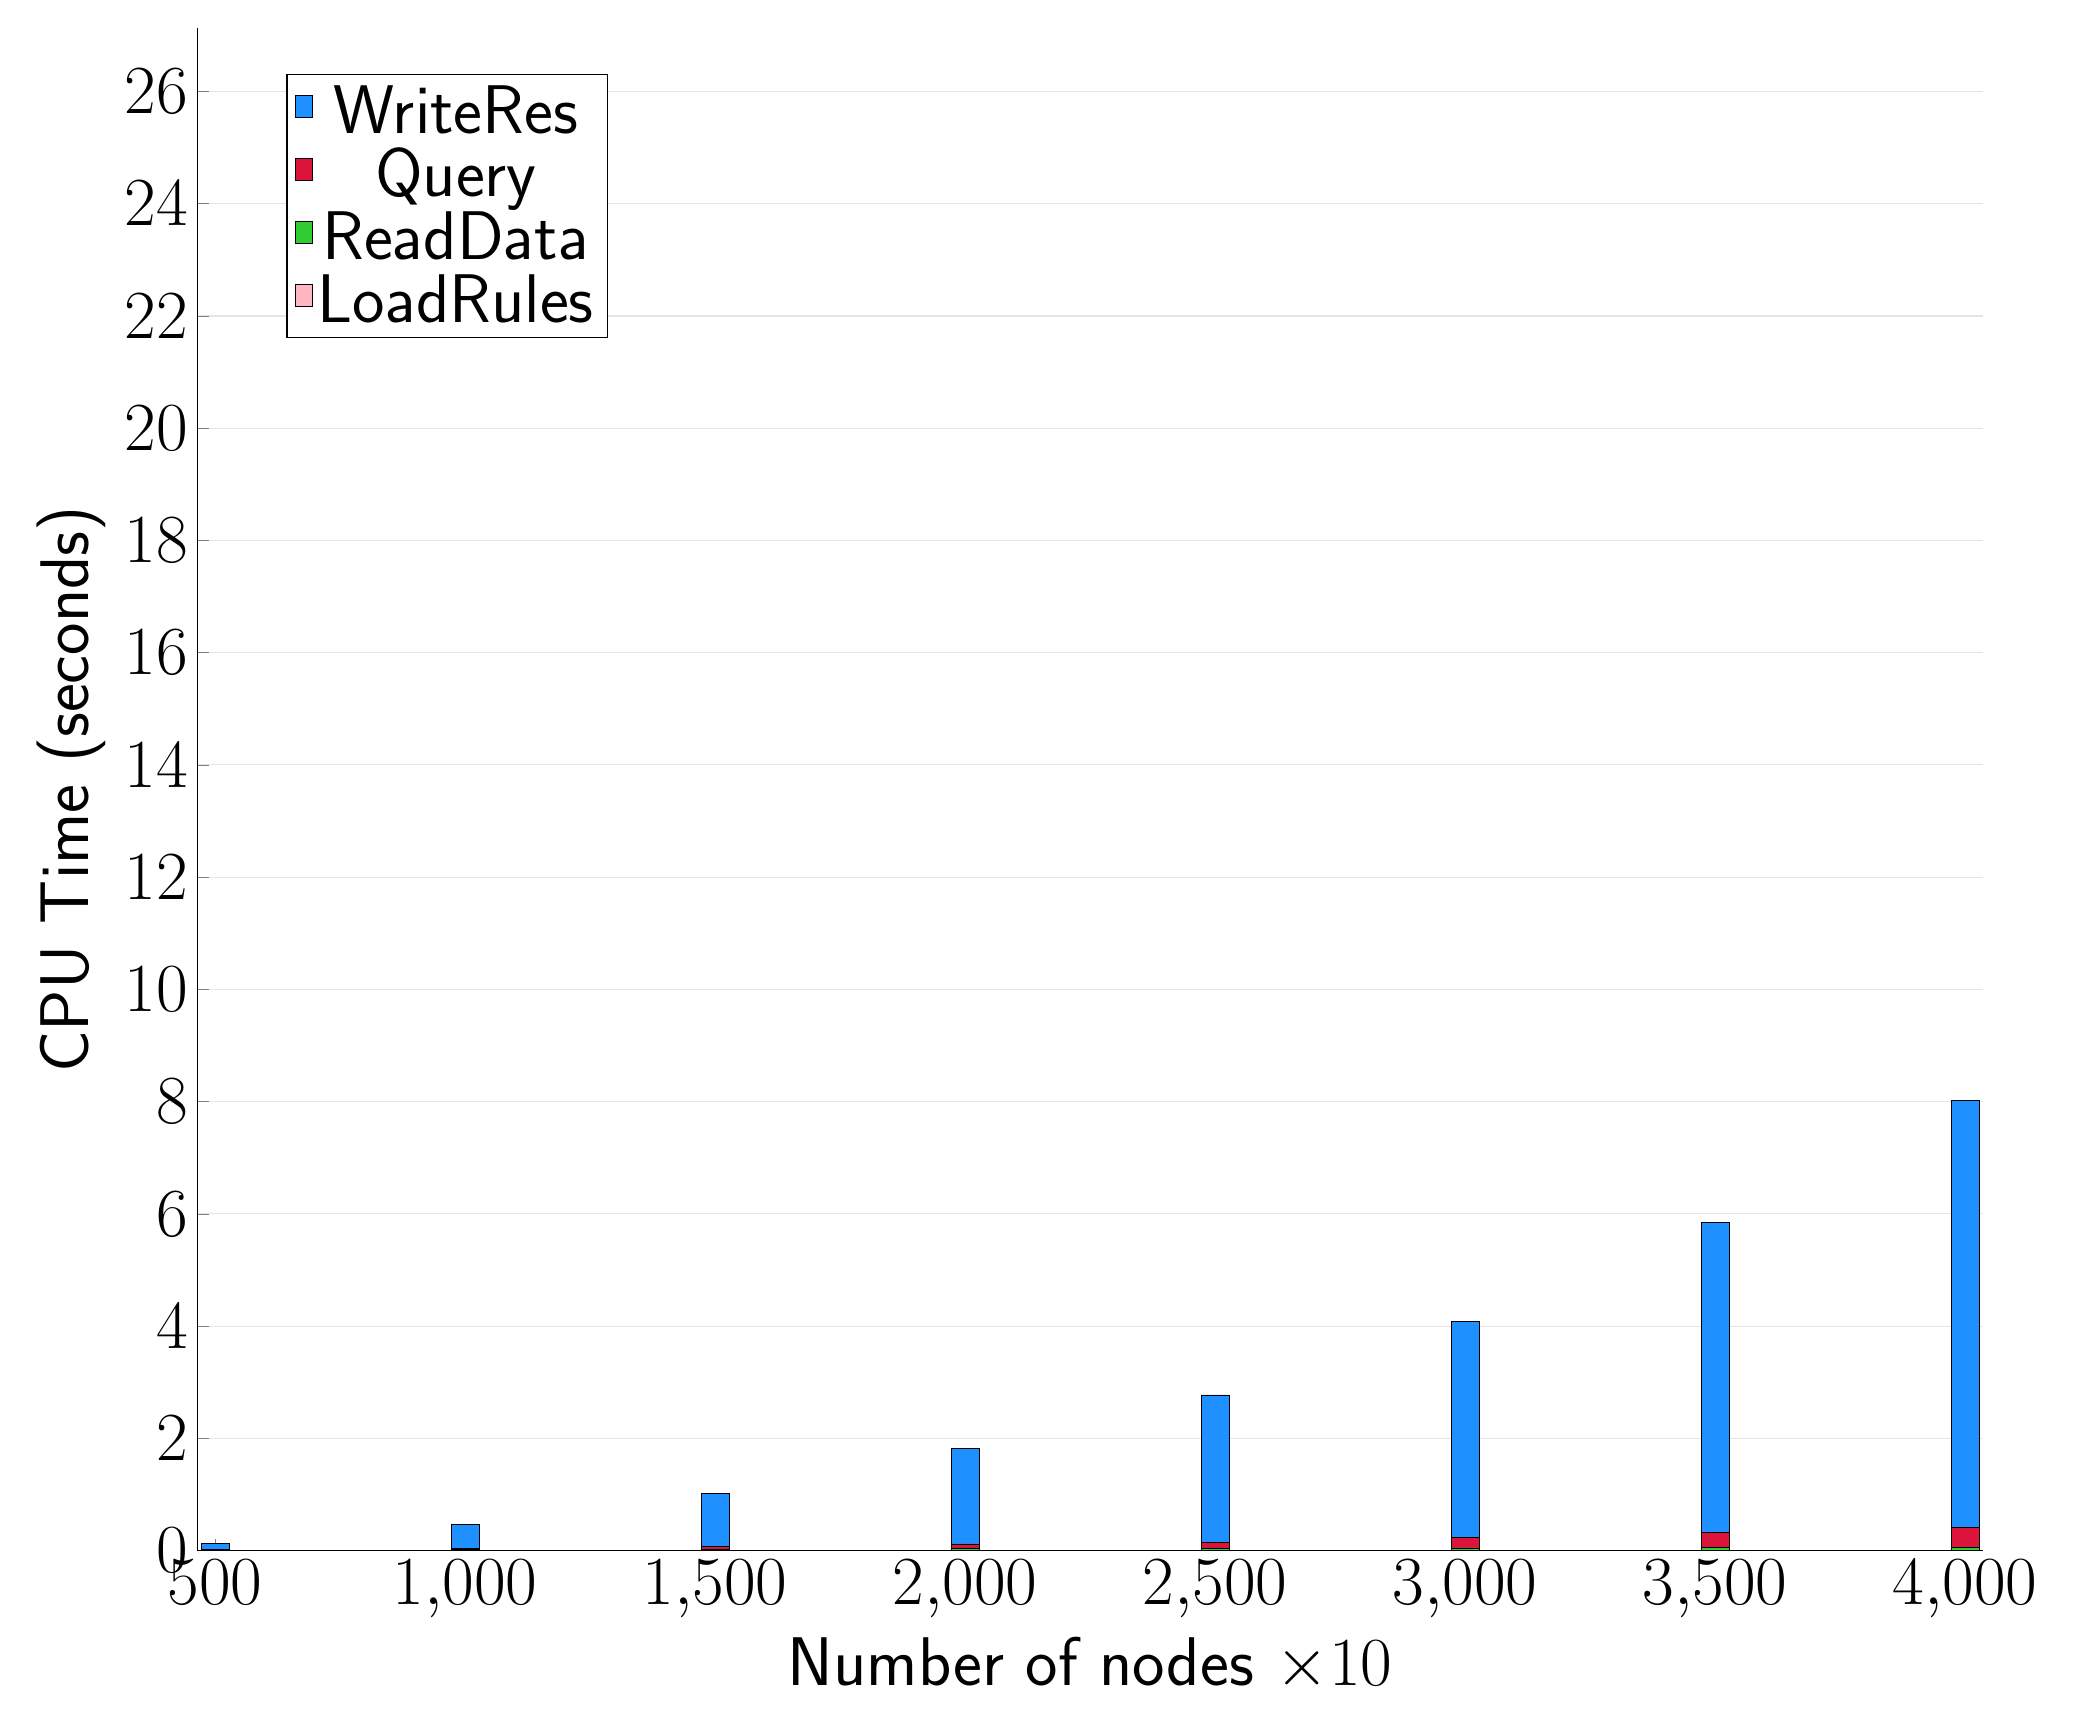
\begin{tikzpicture}
\begin{axis}[
   ybar stacked,
   width=2\textwidth,
   bar width=0.35cm,
   ymajorgrids, tick align=inside,
   major grid style={draw=gray!20},
   xtick=data,
   ymin=0, ymax=27.127176920572918,
   axis x line*=bottom,
   axis y line*=left,
   enlarge x limits=0.01,
   legend style={
       at={(0.23, 0.97)},
       anchor=north east,
       legend columns=1,
       font=\Huge,
   },
   ylabel={CPU Time (seconds)},
   xlabel={Number of nodes $\times 10$},
   label style={font=\Huge},
   tick label style={font=\Huge},
]
\addlegendimage{fill=DodgerBlue, draw=black, line width=0.2pt}
\addlegendentry{WriteRes}
\addlegendimage{fill=Crimson, draw=black, line width=0.2pt}
\addlegendentry{Query}
\addlegendimage{fill=LimeGreen, draw=black, line width=0.2pt}
\addlegendentry{ReadData}
\addlegendimage{fill=LightPink, draw=black, line width=0.2pt}
\addlegendentry{LoadRules}
\addplot +[fill=LightPink, draw=black, line width=0.2pt] coordinates {
(500, 0.005625666666666663)
(1000, 0.004343333333333334)
(1500, 0.004122333333333336)
(2000, 0.003326333333333332)
(2500, 0.003980999999999997)
(3000, 0.003608333333333333)
(3500, 0.004462333333333333)
(4000, 0.004628666666666666)
};
\addplot +[fill=LimeGreen, draw=black, line width=0.2pt] coordinates {
(500, 0.010901)
(1000, 0.01751633333333333)
(1500, 0.024878333333333332)
(2000, 0.032998)
(2500, 0.034127333333333336)
(3000, 0.04551966666666666)
(3500, 0.05416666666666667)
(4000, 0.061450666666666674)
};
\addplot +[fill=Crimson, draw=black, line width=0.2pt] coordinates {
(500, 0.005789666666666663)
(1000, 0.01785233333333333)
(1500, 0.044966)
(2000, 0.08348100000000001)
(2500, 0.113638)
(3000, 0.18485033333333334)
(3500, 0.2631673333333333)
(4000, 0.354875)
};
\addplot +[fill=DodgerBlue, draw=black, line width=0.2pt] coordinates {
(500, 0.114004)
(1000, 0.42601)
(1500, 0.9508220000000001)
(2000, 1.7054456666666666)
(2500, 2.625192333333333)
(3000, 3.849727333333334)
(3500, 5.526930666666666)
(4000, 7.604004666666666)
};
\end{axis}
\end{tikzpicture}

\end{document}
